\documentclass{llncs}

\usepackage{graphicx}
\usepackage{subcaption}
\usepackage{xcolor}
\usepackage[T1]{fontenc}
\usepackage{hyperref}

\graphicspath{ {./img/} }

\begin{document}
\title{Flatland: Malfunctions research on Train Training}
\author{Guillem Gili i Bueno\orcidID{0009-0009-7593-2850}, Felix Mark Kratzsch}
\institute{Universität Potsdam, Am Neuen Palais 10, 14469 Potsdam, Germany}
\date{\today}
\maketitle


\begin{abstract}
The goal of the course is stated as `pushing the boundary of Flatland`.In particular, the goal of our group this semester was to explore further what concepts were necessary/useful regarding malfunctions within the Flatland Framework. In this report, a brief introduction to Flatland is made and the particularities surrounding the usage of malfunctions are highlighted. Then the sets of environments that were found the most interesting for the sake of benchmarking are explained, followed by the solutions that we decided to test for these environments. A comparison is drawn between using solutions that are more reutilization friendly than others. Finally, the results are summarized and  we conclude 
\color{green} BLABLALABLBA CONCLUSIONS \color{black}

\keywords{ASP \and Multi-Agent Pathfinding \and Resilience planning.}
\end{abstract}

\setcounter{tocdepth}{4}
\tableofcontents


\section{Introduction to Flatland and Malfunction mechanics}

\subsection{Flatland}
Flatland\cite{flatland} is the framework this report researches on. To quote from the official repository:
\begin{quote}
\emph{	Flatland is a railway scheduling challenge hosted by AICrowd that seeks to solve the problem of multi-agent pathfinding for trains in large railway networks. Although approaches across all domains (e.g. reinforcement learning, operations research) are welcome, this repository focuses on integrating ASP-based solutions within the Flatland framework.}
\end{quote}

The simulation environment allows specific connections between different roads, different train speeds and for unexpected malfunctions. As the title of this report alludes to, we will be focusing on the more malfunction-adjacent implications, and measuring across various aspects that may be related to it.

\color{green}
\begin{itemize}
	\item personal horizons as estimates
	\item ignore horizons
\end{itemize}
\color{black}

\subsection{Particularities of malfunctions}
\color{green}
\begin{itemize}
	\item what are primary and secondary encodings? Are used later but a short explanation would be neat
\end{itemize}
\color{black}
A flatland simulation is run one step at a time, meaning that a train of the max speed, 1, which is also the default, will advance to a the next cell in the direction it is facing. At run-time, a malfunction (or multiple) may happen at any point. A malfunction at time T, with duration D implies the train must wait during D turns (or if it is unspawned, it must remain that way), from turn T onward. To be very precise: the action performed in T-1 will be completed (so a change of coordinates may happen between T-1 and T) but the action that is started at T must be `wait`. This will turn valid solutions into invalid; and force trains to arrive later. This translates roughly to 2 things:
\begin{itemize}
	\item Figure out the commited atoms until the point where a malfunction happened.
	\item Rerun the problem solution, inheriting commited choices\footnote{In the current implementation of Flatland, the problem basic atoms must also be forwarded `start/4`, `end/3` and `train/1`}, and adding the malfunctioning actions.
\end{itemize}
During the semester the `save/1`  and `load/1` atoms were added \cite{malfunction_branch}, so that the atoms from a previous solution that incurred into a malfunction were inherited into a new, recalculated solution. \color{green} They are single-argument (rather than something time-related, making it a 2-argument) to allow for more flexibility; this way one can store full atoms directly. This makes `primary` and `secondary` encondings in flatland now relevant to differentiate; one can now store the base-structure representation so it does not need to be recalculated. \color{black} \color{gray} I find this confusing. I would call the predicates unary and think flexibility as it stands here unexplained. Just confuses. I would just cut it like: They are unary predicates but due to Clingos nature can store unlimited complex structures. \color{black}

\section{Core malfunctions analysis / particularities}

\color{green}
\subsection{Definitions}
To not reiterate the descriptions of the example files we are using for our properly-structured solution, I will be describing it here. While our solution is graph-based; it should be valid for other approaches. The respective files are:
\begin{itemize}
	\item  \textbf{input.lp} File that generates the base problem representation (a graph or other); with no choice rules.
	\item  \textbf{path.lp} File that uses choice rules to determine the path.
	\item  \textbf{output.lp} File that deduces, given the elected path, which action should be followed by each train; with no choice rules.
	\item  \textbf{malfunctions.lp} File that loads (selectively, according to the timestamp) and saves upon malfunction. Also where path implications from a malfunction should be deduced; with no choice rules.
\end{itemize}
\color{black} \color{gray} I would get rid of this. I think our structure is not important, as it adds nothing to the execution, for the order of lines does not matter. \color{black}
\color{blue}
\begin{itemize}
	\item make small section for it
	\item flatland and action saving and state machine problems
\end{itemize}
\color{black}


\subsection{Implications on Encodings}
\color{green}
\subsubsection{Modularity}
A common issue when debugging and ASP problem is to figure out which choice rules or deductions may be the biggest timesink in your program. To debug this is usually complicated, and will in all likelyhood disencourage someone unfamiliar with the particularities of grounding and what is used beyond syntax. To draw a simile, I may not know all the secrets of a C++ compiler, but I can write a mediocre C++ code, with timestamps that allow me to figure what particular part of my program is slow, then iterate an improve. This is the case for most programming languages, but no such straightfoward approach exists on `clingo`.

By being allowed to selectively load a set of atoms (that have been generated dynamically), we can easily identify which atom generation is slowing down the program. Doing this is far from the most common way to debug these issues in your average clingo program, but it does respect the fact that clingo wants the solver to be solution-agnostic. 
\color{black} \color{gray} I would make this just a small note, as it has nothing to do with the problem. And maybe add it to the back if this section. \color{black}
\subsubsection{File structure}
\color{green}
As one may deduce from the different primary/secondary set of encodings, this means a problem representation will have a set of files that is used only for the first run(that only saves) and another for each subsequent malfunction(that saves and loads). As an interesting factor to take into account, we test later on `naive` vs. `proper` approaches; as one could naively use the union of the entire set of files for both approaches. We have chosen to follow these general guidelines for our proper approaches:
\begin{itemize}
	\item  \textbf{Saves for an atom are done on the same file it is deduced} Implying that `input.lp` must save the base problem representation. Choice-rule derived atoms are saved in `path.lp` and no saving is needed on `output.lp`. 
	\item  \textbf{Base-problem save requirements are done on `path.lp`} As they need to be forwarded always, they behave akin to choice-rule derived atoms.  
	\item  \textbf{Load only in `malfunctions.lp`}  Since load statements are only useful in the event of a malfunction; they are done there. 
\end{itemize}
\color{black} \color{gray} I think this is to complicated. Also as of now, we only have one encoding with a "naive" implementation. I think the explanation is to methodical and also my "naive" version doesn't fit in. I would just give it a section and don't put it here in this general fashion. \color{black}
\subsubsection{Window of grounding}

\subsection{Our interests}
We found it likely that 2 approaches made sense:
\color{green}
\begin{itemize}
	\item get running baseline 
	\begin{itemize}
		\item reschedule
	\end{itemize}
	\item three focuses
	\begin{itemize}
		\item try different structure
		\begin{itemize}
			\item subcellid\_proper
			\item your encoding if we want to
		\end{itemize}
		\item don't pass info
		\begin{itemize}
			\item reschedule\_naive
		\end{itemize}
		\item deal with the window (less timesteps)
		\begin{itemize}
			\item incremental
		\end{itemize}
	\end{itemize}
\end{itemize}
\color{black}


\section{Solutions}

\subsection{Naive (vertex with directions) file partition}
malfunctions + main
\color{blue}
\begin{itemize}
	\item motivation (comparison of passing and recomputing)
	\item implementation
	\begin{itemize}
		\item just adding malfunction handling on top
		\item passing just basic information
	\end{itemize}
	\item implications
	\begin{itemize}
		\item slower grounding?
		\item else similar as just reschedule
	\end{itemize}
\end{itemize}
\color{black}


\subsection{Smart (vertex with directions) file partition}
\color{green} Would make this one the first, as it is the easiest to explain. And easy to narrate as we implemented it. \color{black}
malfunctions + input+ path+output
\color{blue}
\begin{itemize}
	\item motivation
	\item implementation
	\begin{itemize}
		\item short summary on graph structure
		\item talk about split (whats primary, whats secondary)
		\item extending the window (worst case assumption)
	\end{itemize}
	\item implications
	\begin{itemize}
		\item escalating window
		\item bad scaling
		\item quick with good estimates
	\end{itemize}
\end{itemize}
\color{black}

\subsection{Incremental}
\color{blue}
\begin{itemize}
	\item motivation (better window)
	\item implementation
	\begin{itemize}
		\item work clingo side
		\item solving adaptations
		\item step splitting
		\item primary secondary split
	\end{itemize}
	\item implications
	\begin{itemize}
		\item sometimes slower
		\item faster overall
		\item more adaptive (theoretically does not require horizon)
	\end{itemize}
\end{itemize}
\color{black}


\section{Results}
\section{Instances}
\color{green} Would move it to a testing section right before evaluation \color{black}\\
sparse\_0\_1 means sparse with 0\% malfunctions the first one.
\color{blue}
\begin{itemize}
	\item would make it a testing section
	\item explain instances (why how, ...)
	\item explain benchmarking (how, why, ...)
\end{itemize}
\color{black}

\subsection{Sparse instances}

\begin{figure}	
	\begin{minipage}{.41\textwidth}
		\begin{subfigure}{\textwidth}
			\centering
			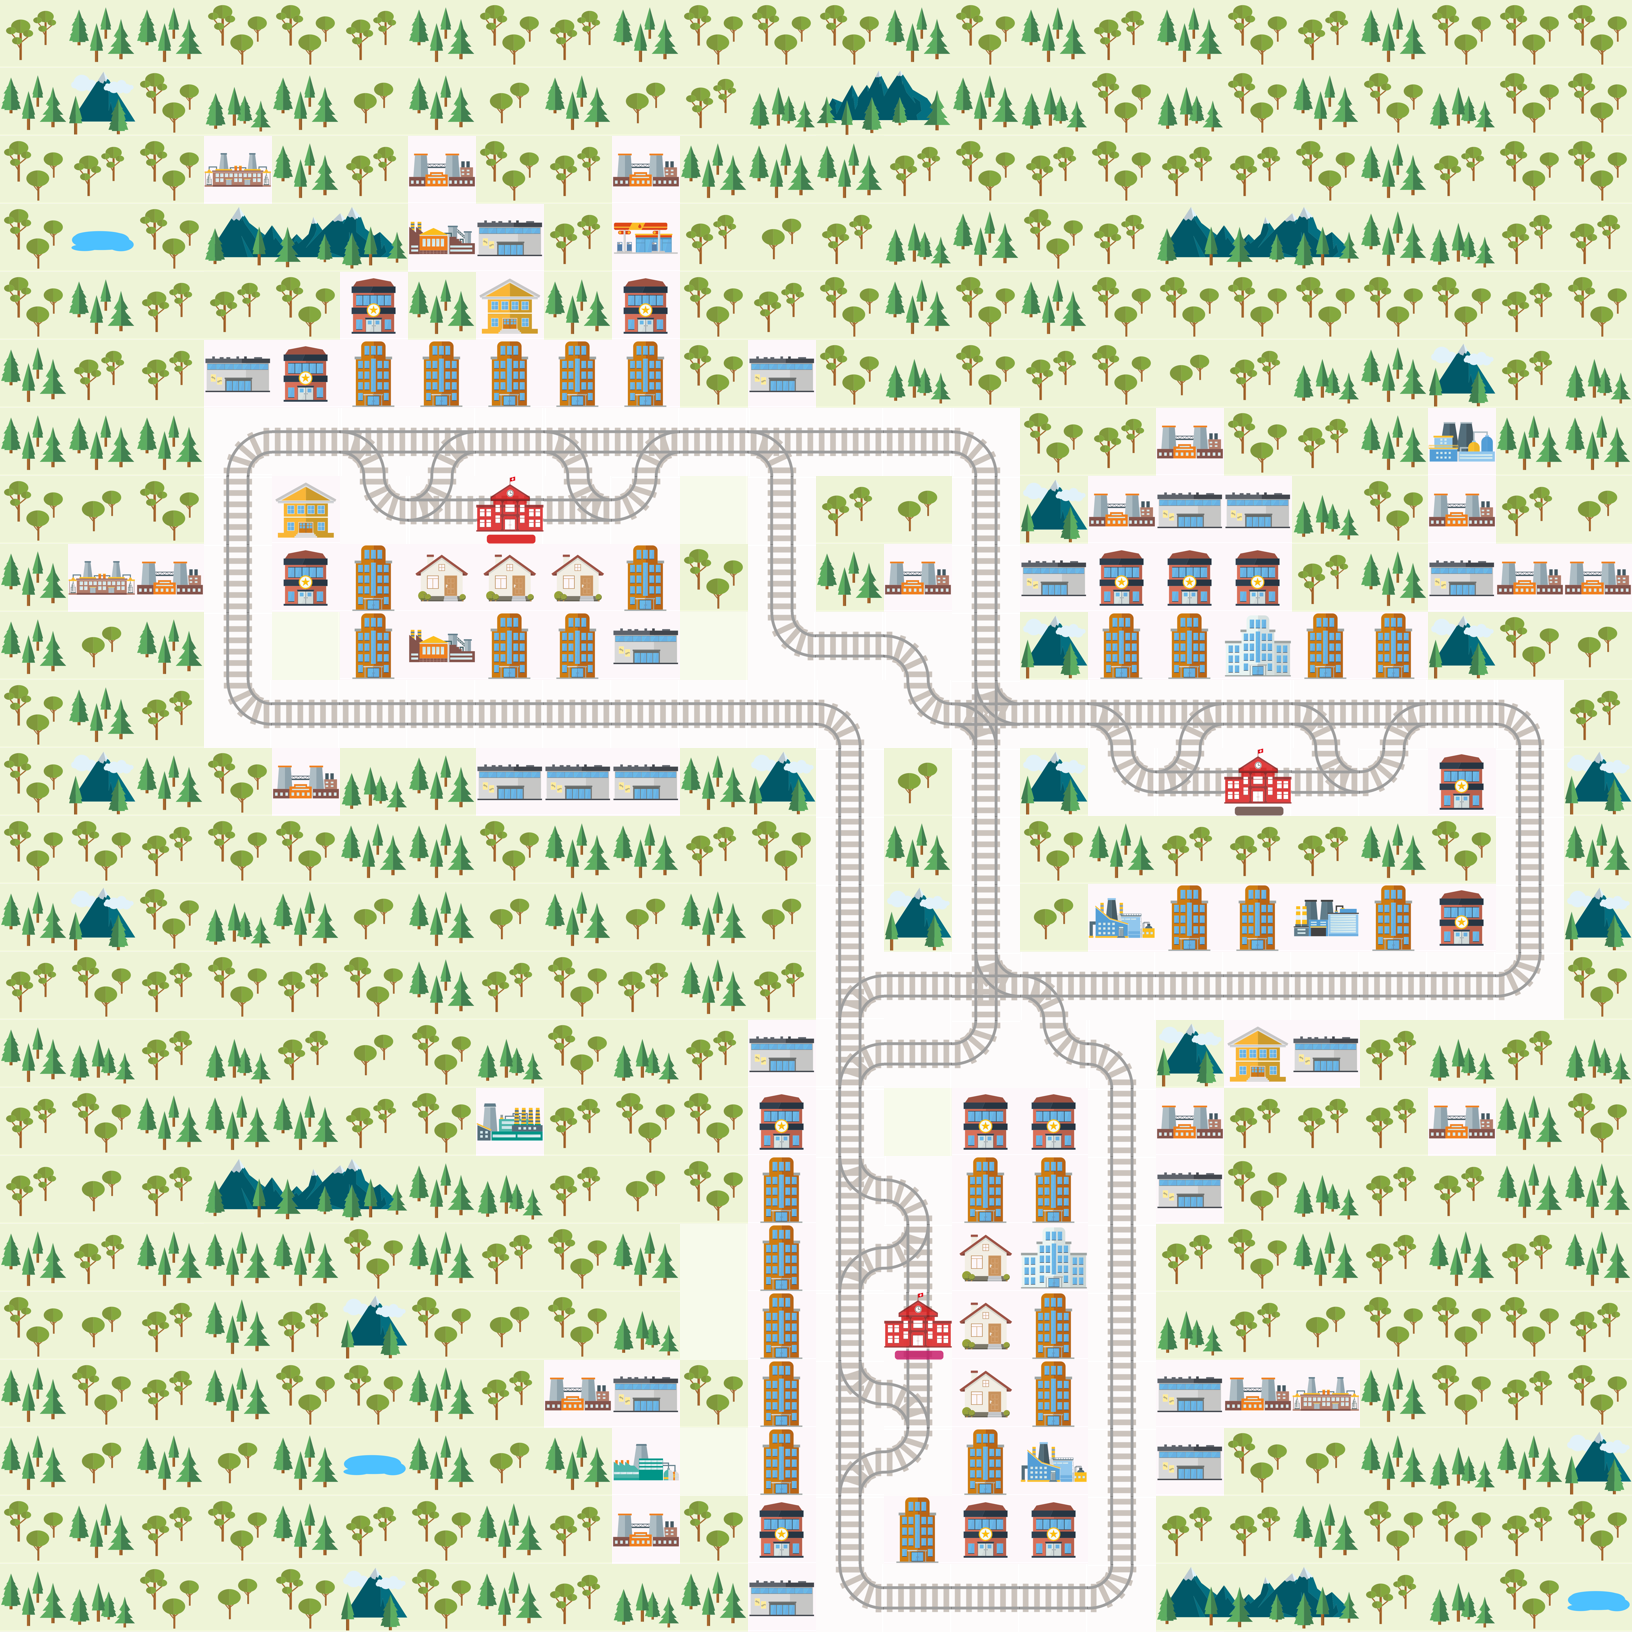
\includegraphics[width=0.48\textwidth]{dense/dense_0_1}
			\caption{Dense instance, using a 24x24 grid, where 20 trains must travel across 3 cities.}
			\label{dense_0_1}
		\end{subfigure}
	\hfill
		\begin{subfigure}{\textwidth}
			\centering
			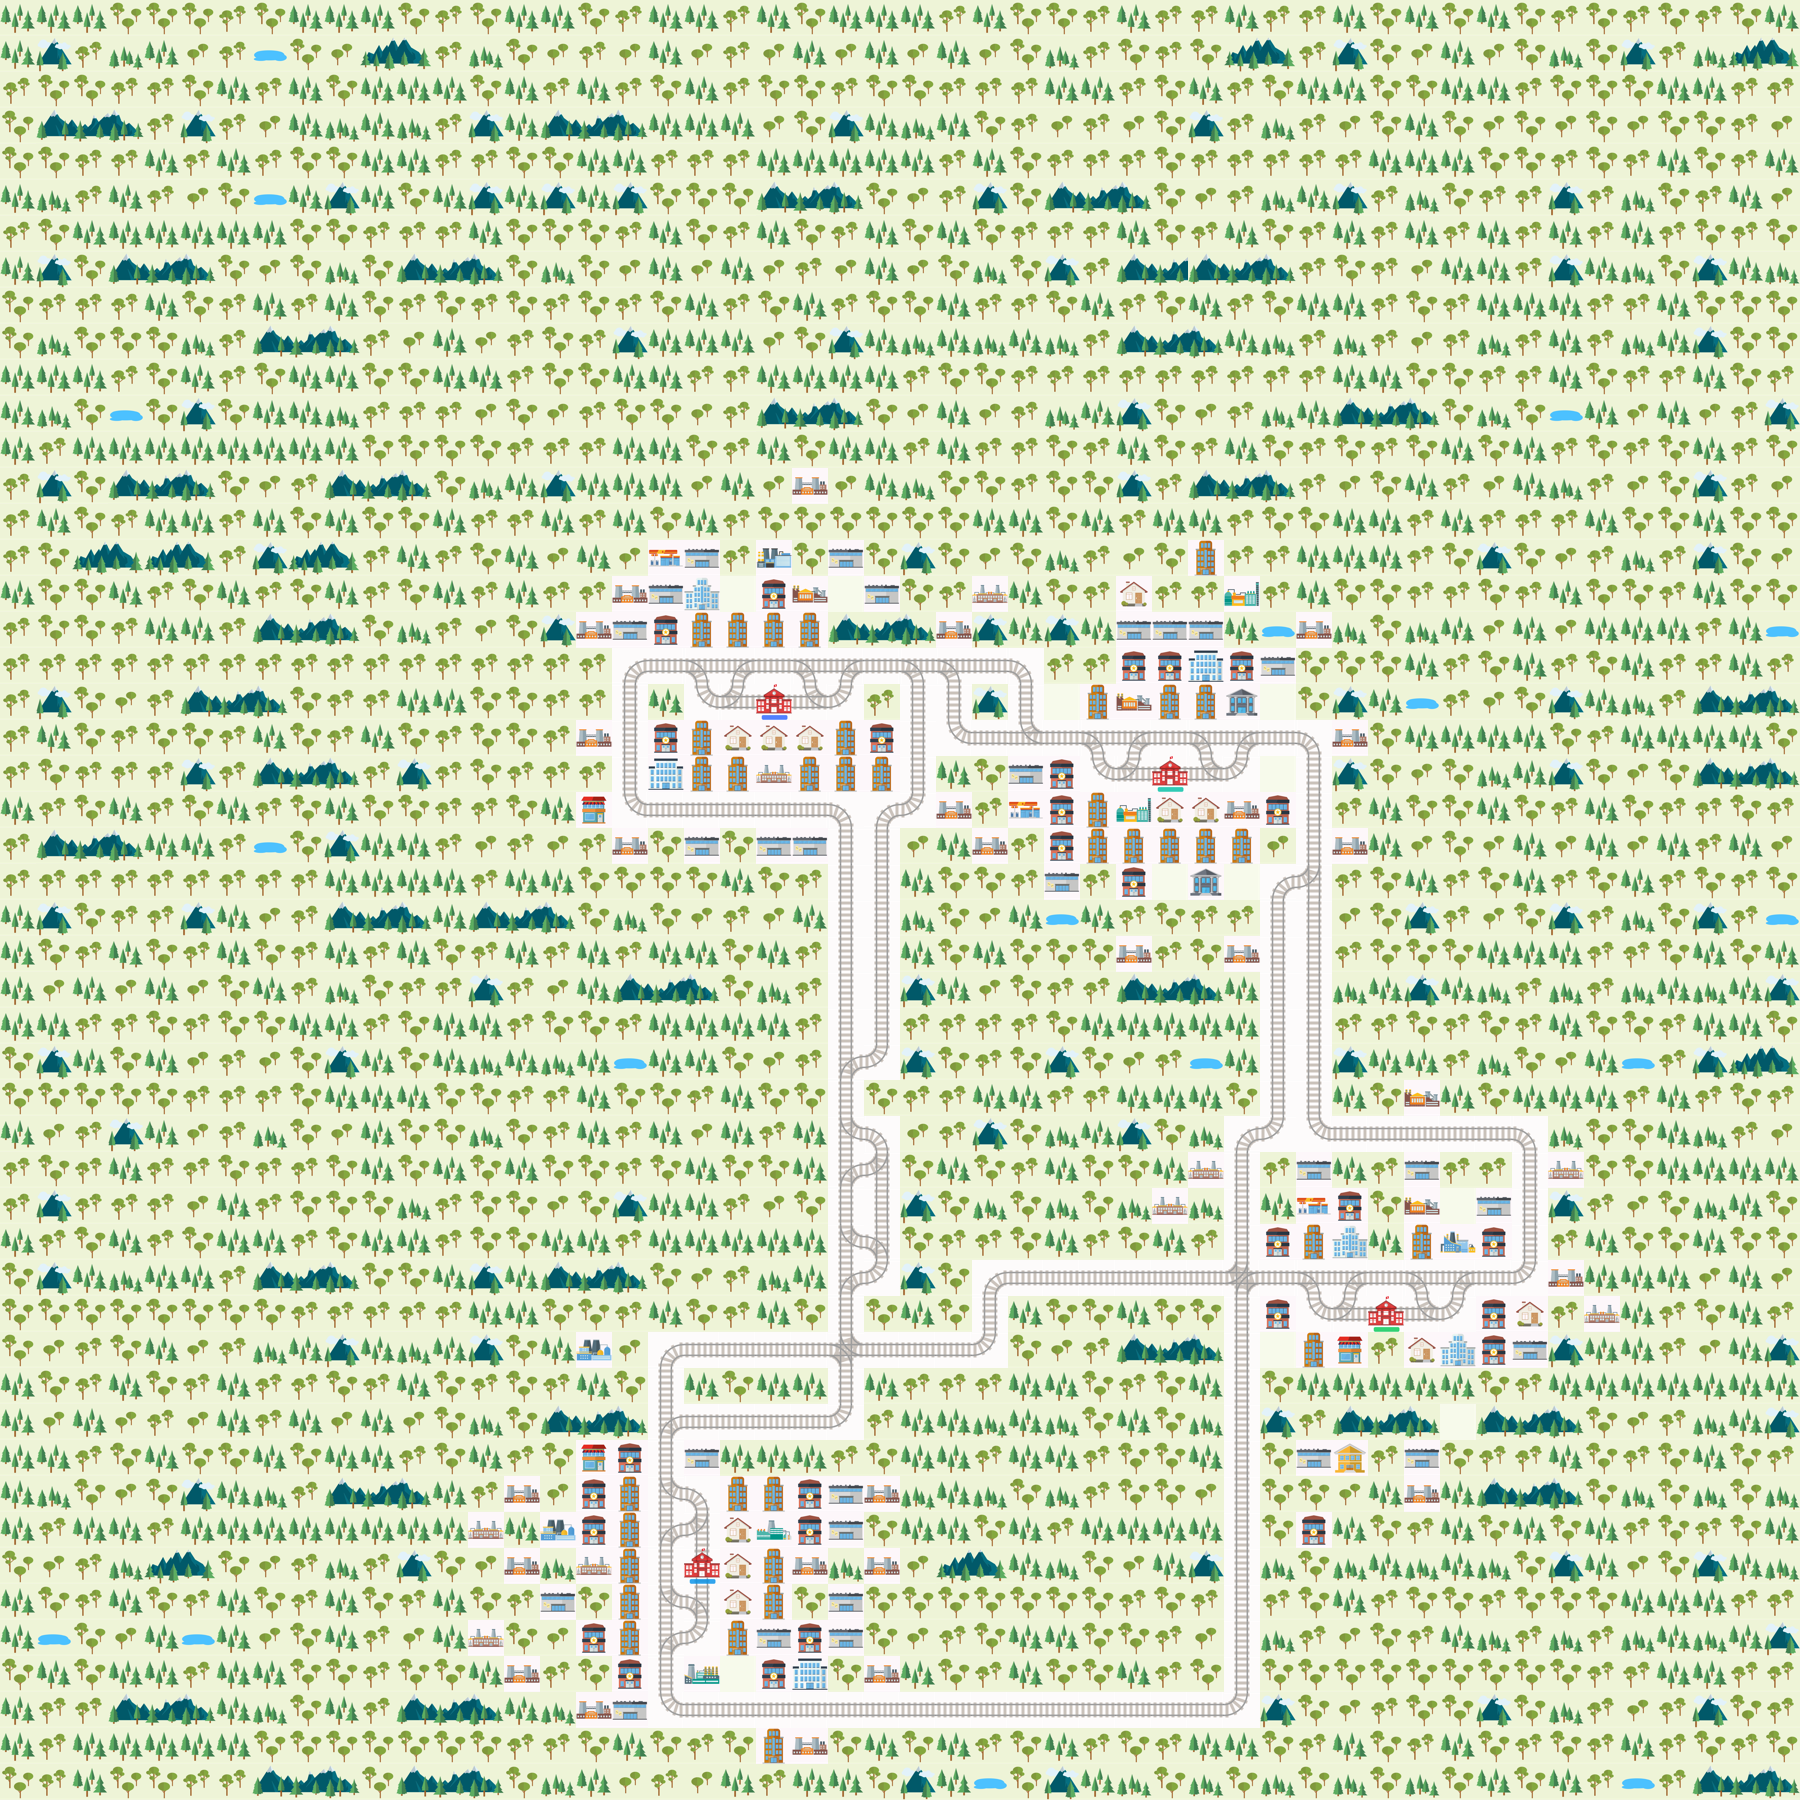
\includegraphics[width=\textwidth]{medium/medium_0_1}
			\caption{Medium instance, using a 50x50 grid, where 10 trains must travel across 5 cities.}
			\label{medium_0_1}
		\end{subfigure}
	\end{minipage}
	\hfill
	\begin{minipage}{.49\textwidth}
				\begin{subfigure}{\textwidth}
		\centering
		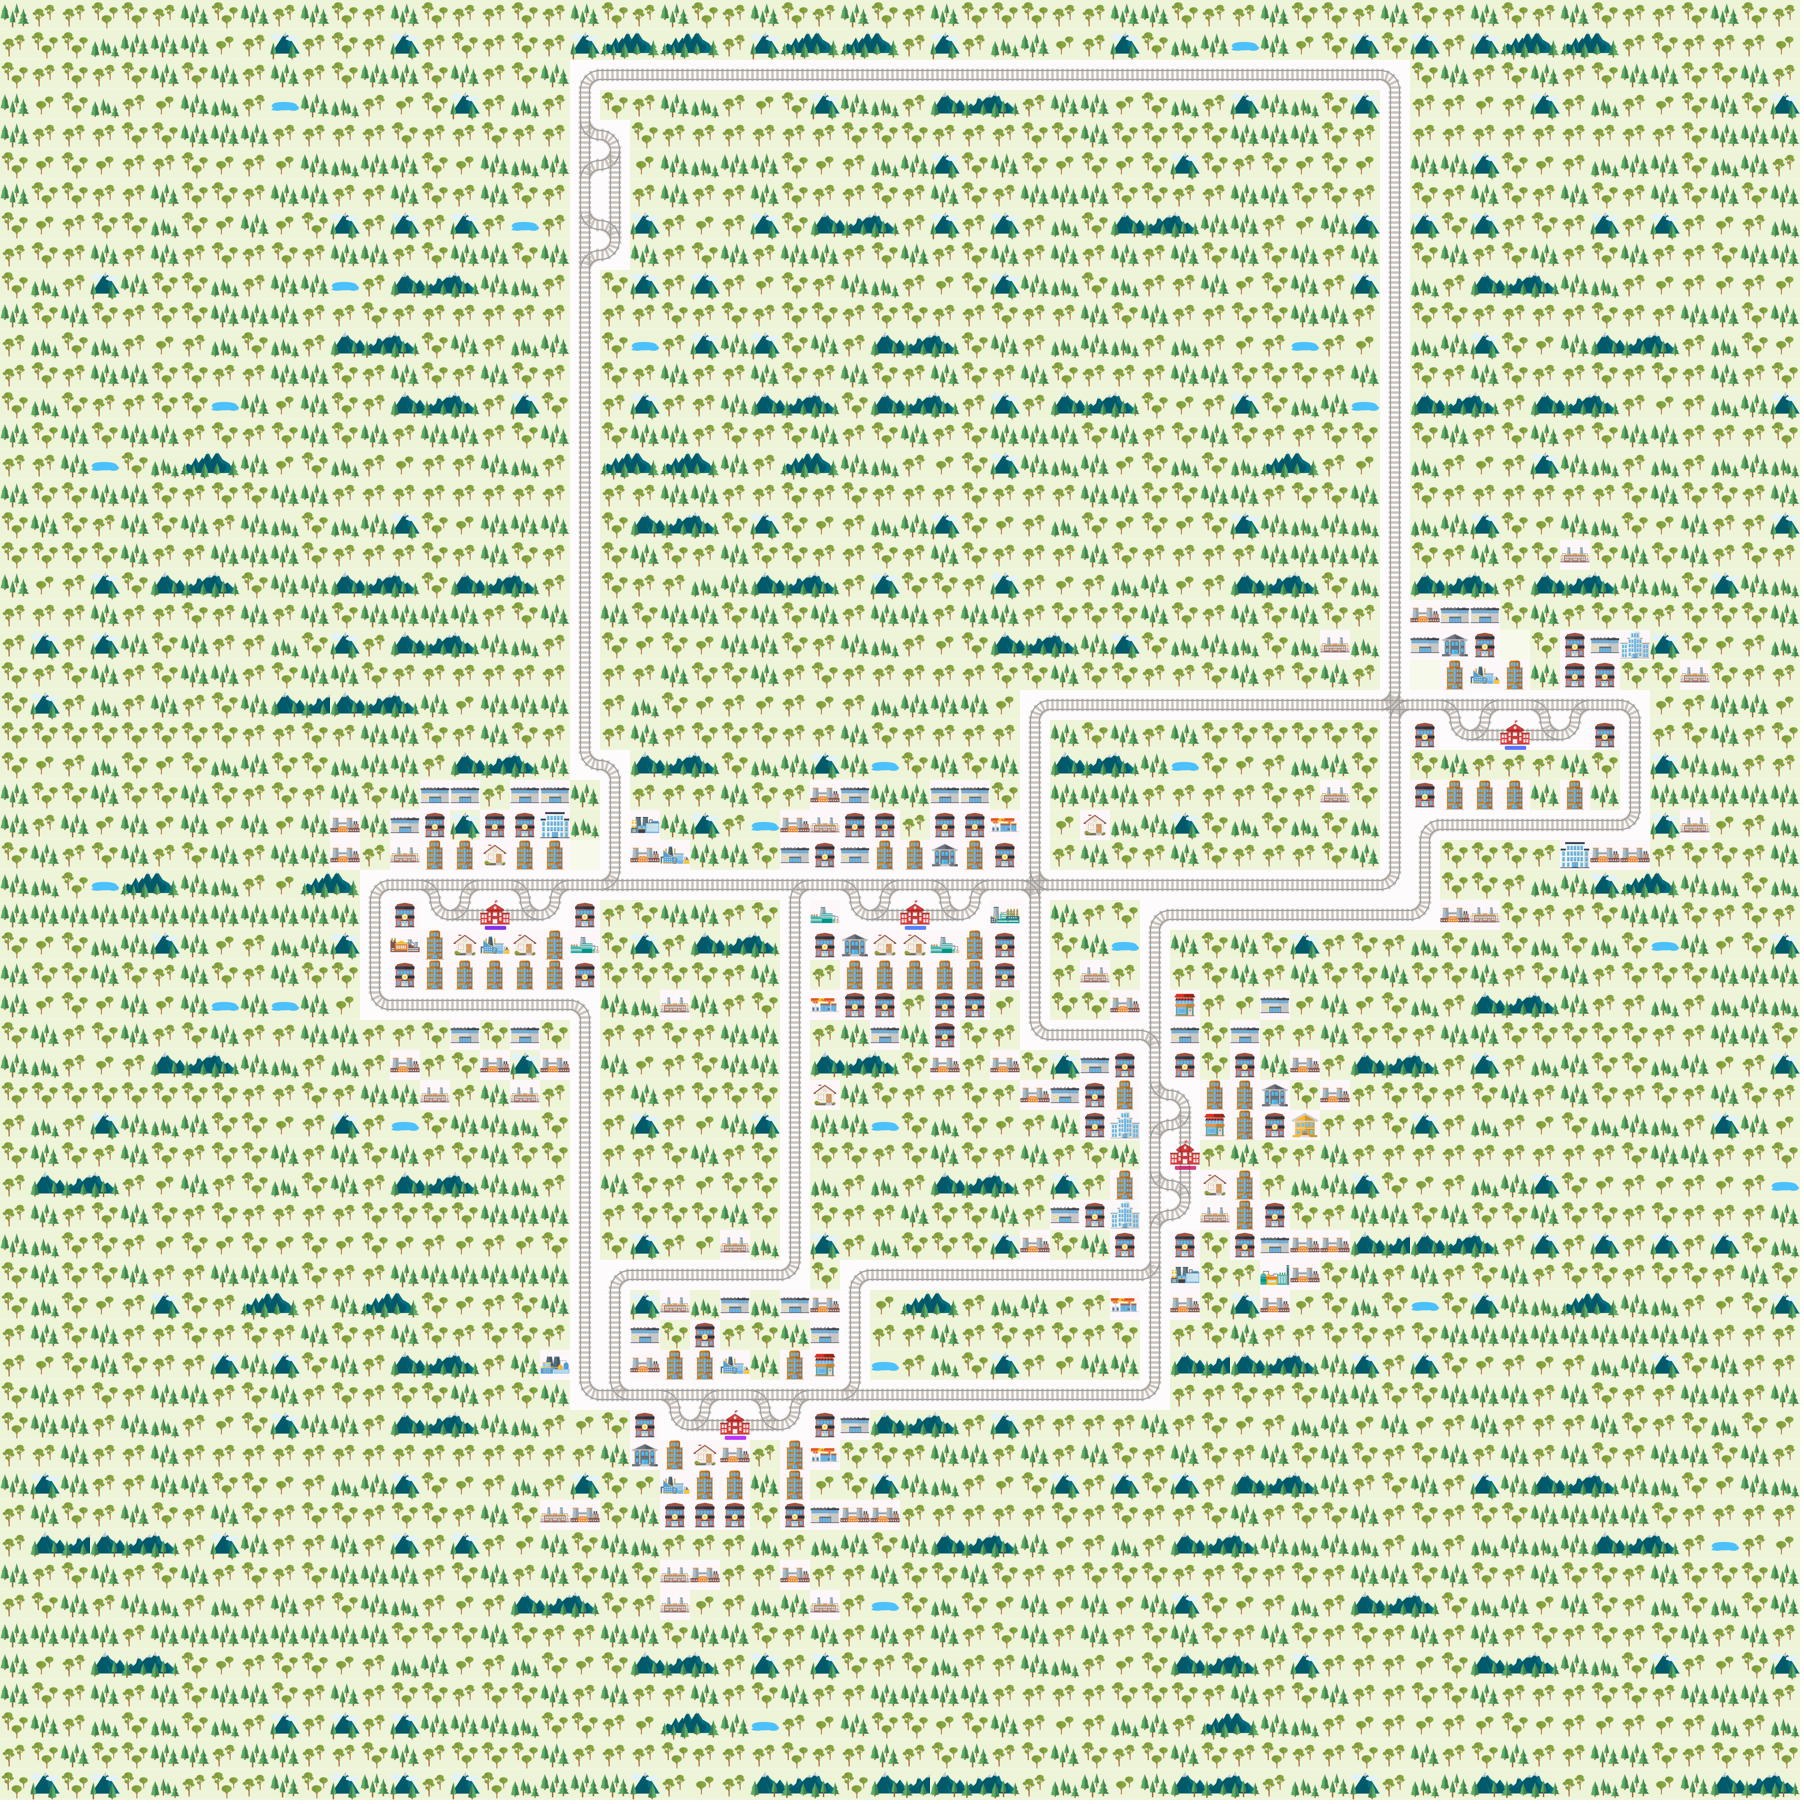
\includegraphics[width=\textwidth]{sparse/sparse_0_1}
		\caption{Sparse instance, using a 60x60 grid, where 6 trains must travel across 6 cities.}
		\label{sparse_0_1}
				\end{subfigure}
	\end{minipage}
	\caption{The 3 types of configurations used for our experimentation, put side-by-side in order to get an idea of the scale. The full list can be found at \cite{instance_folder}}
	\label{sparse_medium_dense}
\end{figure}

\subsection{Medium instances}

\subsection{Dense instances}



\section{Conclusions}
\color{blue}
\begin{itemize}
	\item check hypothesis from encodings
	\item some overall stats (might do later) (space, time, ...)
\end{itemize}
\color{black}

\color{green}
\begin{itemize}
	\item research options
	\item optimality, priority, resilience (need for malfunction handling)
\end{itemize}
\color{black}
\color{green}
\begin{itemize}
	\item  \textbf{Evaluate for optimal solutions} Add a prioritize statement, that ensures trains arrive with as much free time as possible . After a malfunction, the pruned solutions are likely to be the suboptimal.(less efficiency, more resilience)
	\item  \textbf{Evaluate for quick, scalable solutions} Do not do any prioritization; since the solution space is very big. Find solutions as they appear. This may seem naive, but in a real-world case scenario, where the horizon of actions can be infinite(and the time value span much bigger)  there is a good case for this to be a priority. (more (inmediated)efficiency, less resilience )
\end{itemize}
\color{black}


\section{Personal observations}
In order to prioritize the malfunctions specific study, I choose to be rather brief with my overall introduction to flatland, as was also requested for the presentation


\bibliographystyle{splncs04}
\bibliography{report}{}


\appendix
\clearpage
\section{Appendix}
\label{sec:appendix}

\begin{figure}[h]
	
	\centering
	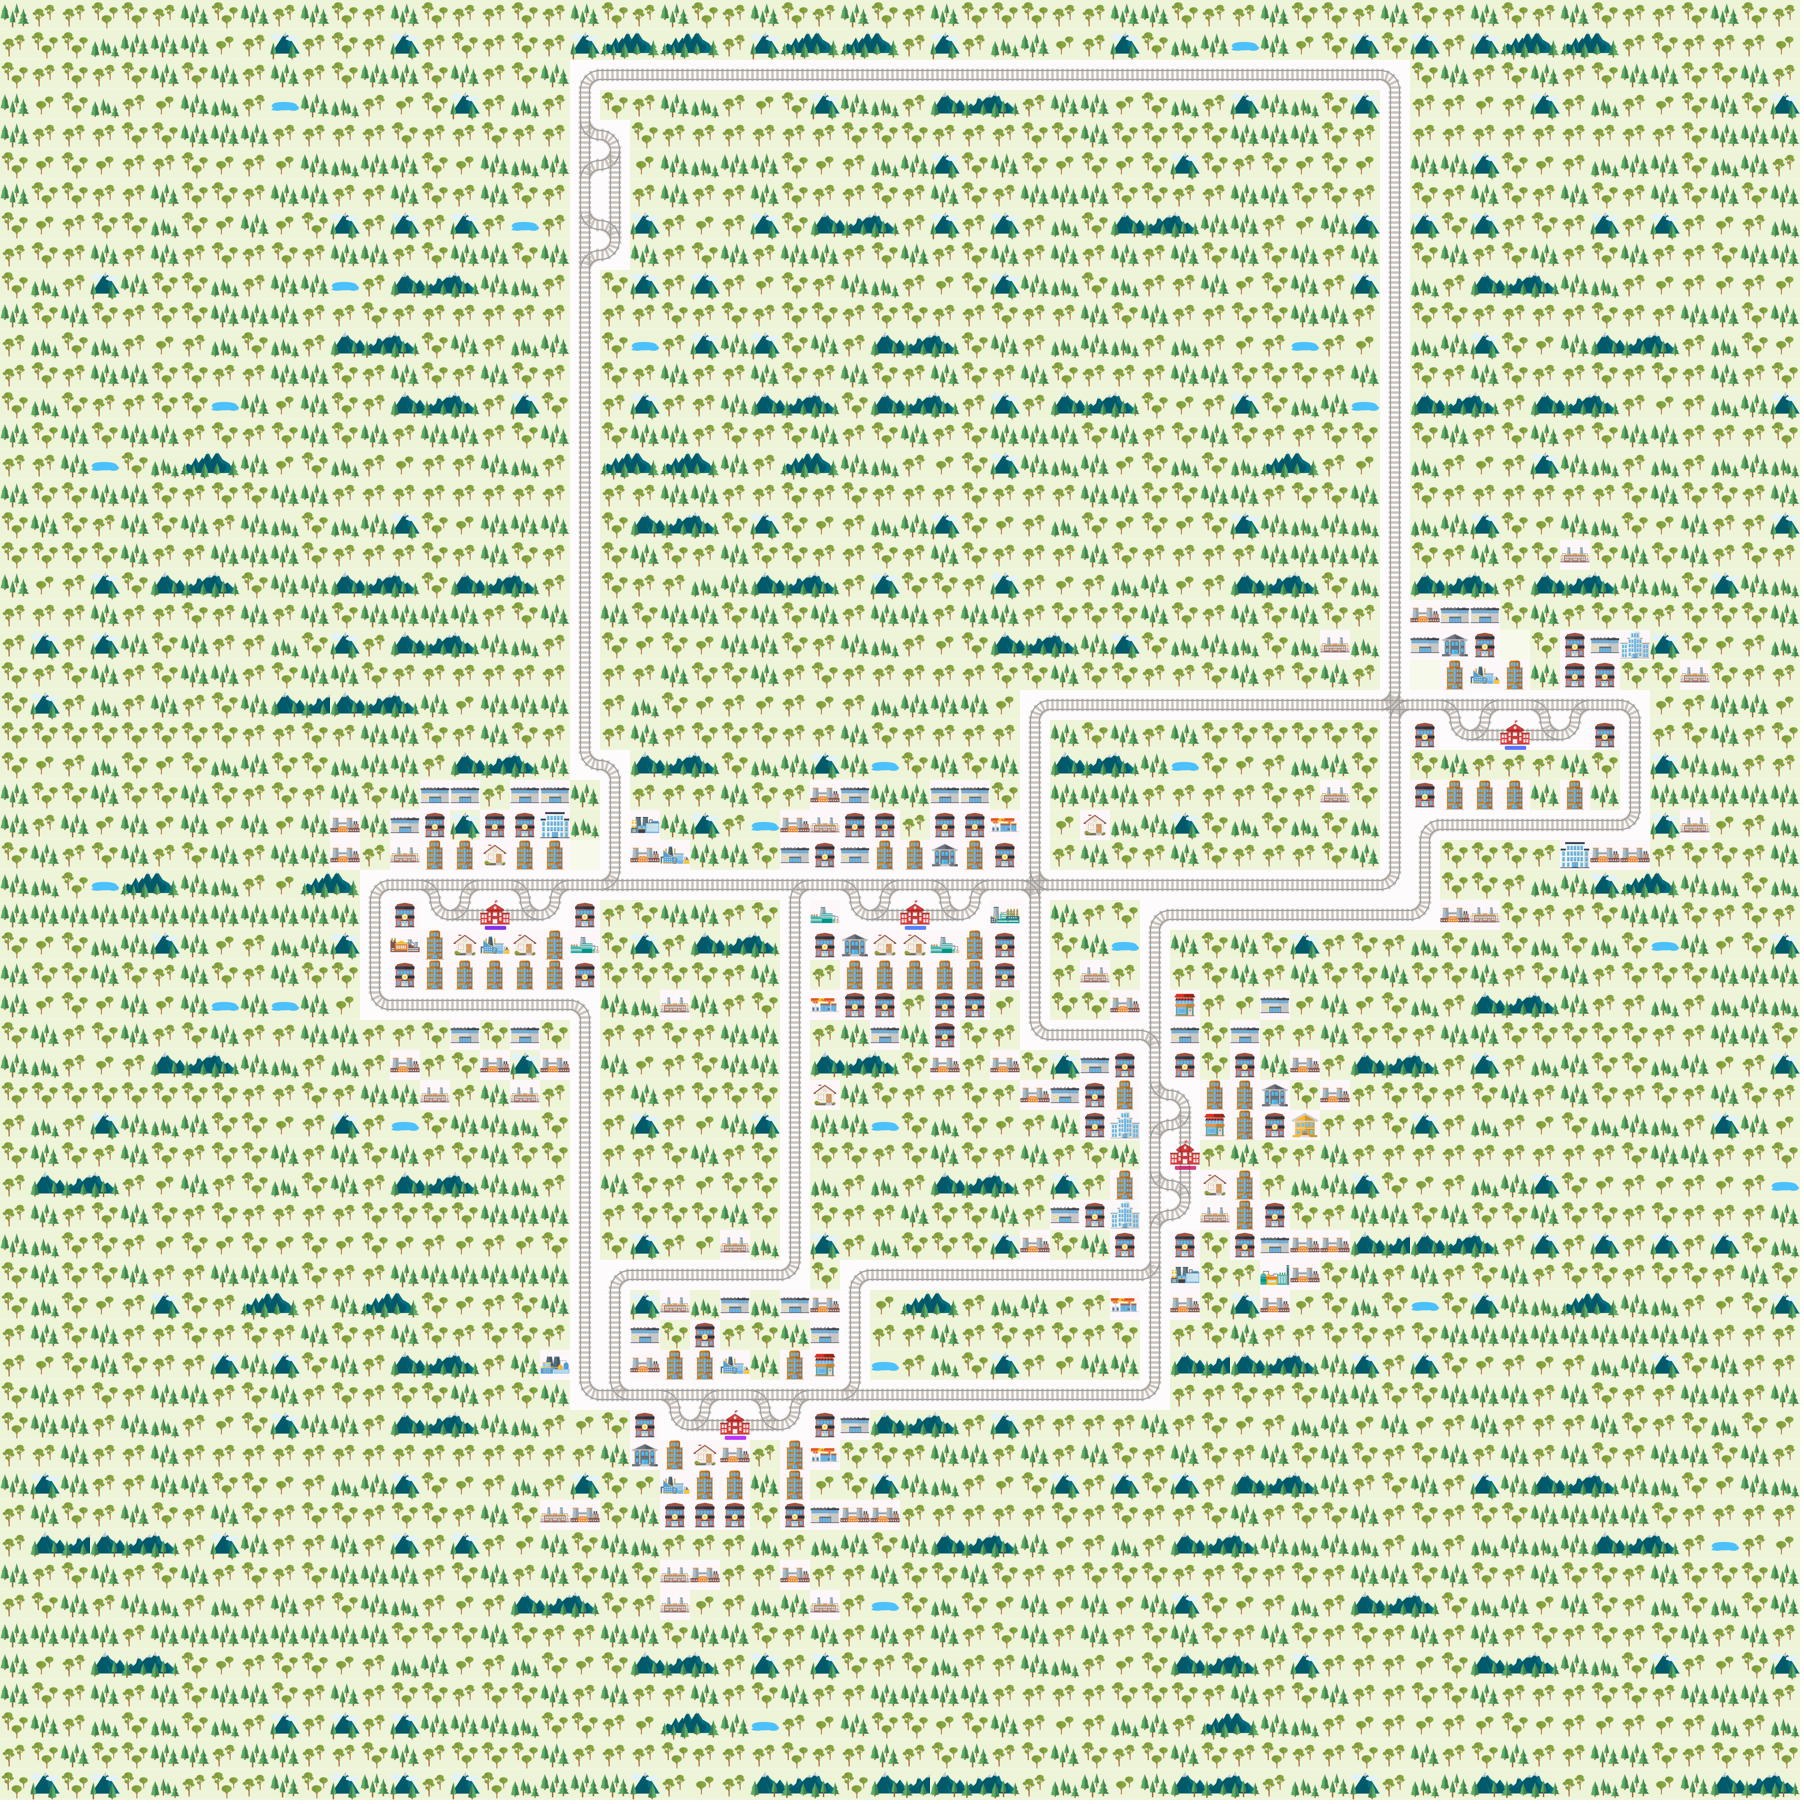
\includegraphics[width=0.9\textwidth]{sparse/sparse_0_1}
	\caption{Sparse instance, using a 60x60 grid, where 6 trains must travel across 6 cities.}
	\label{sparse_0_1_fullpage}
\end{figure}

\begin{figure}[h]
	
	\centering
	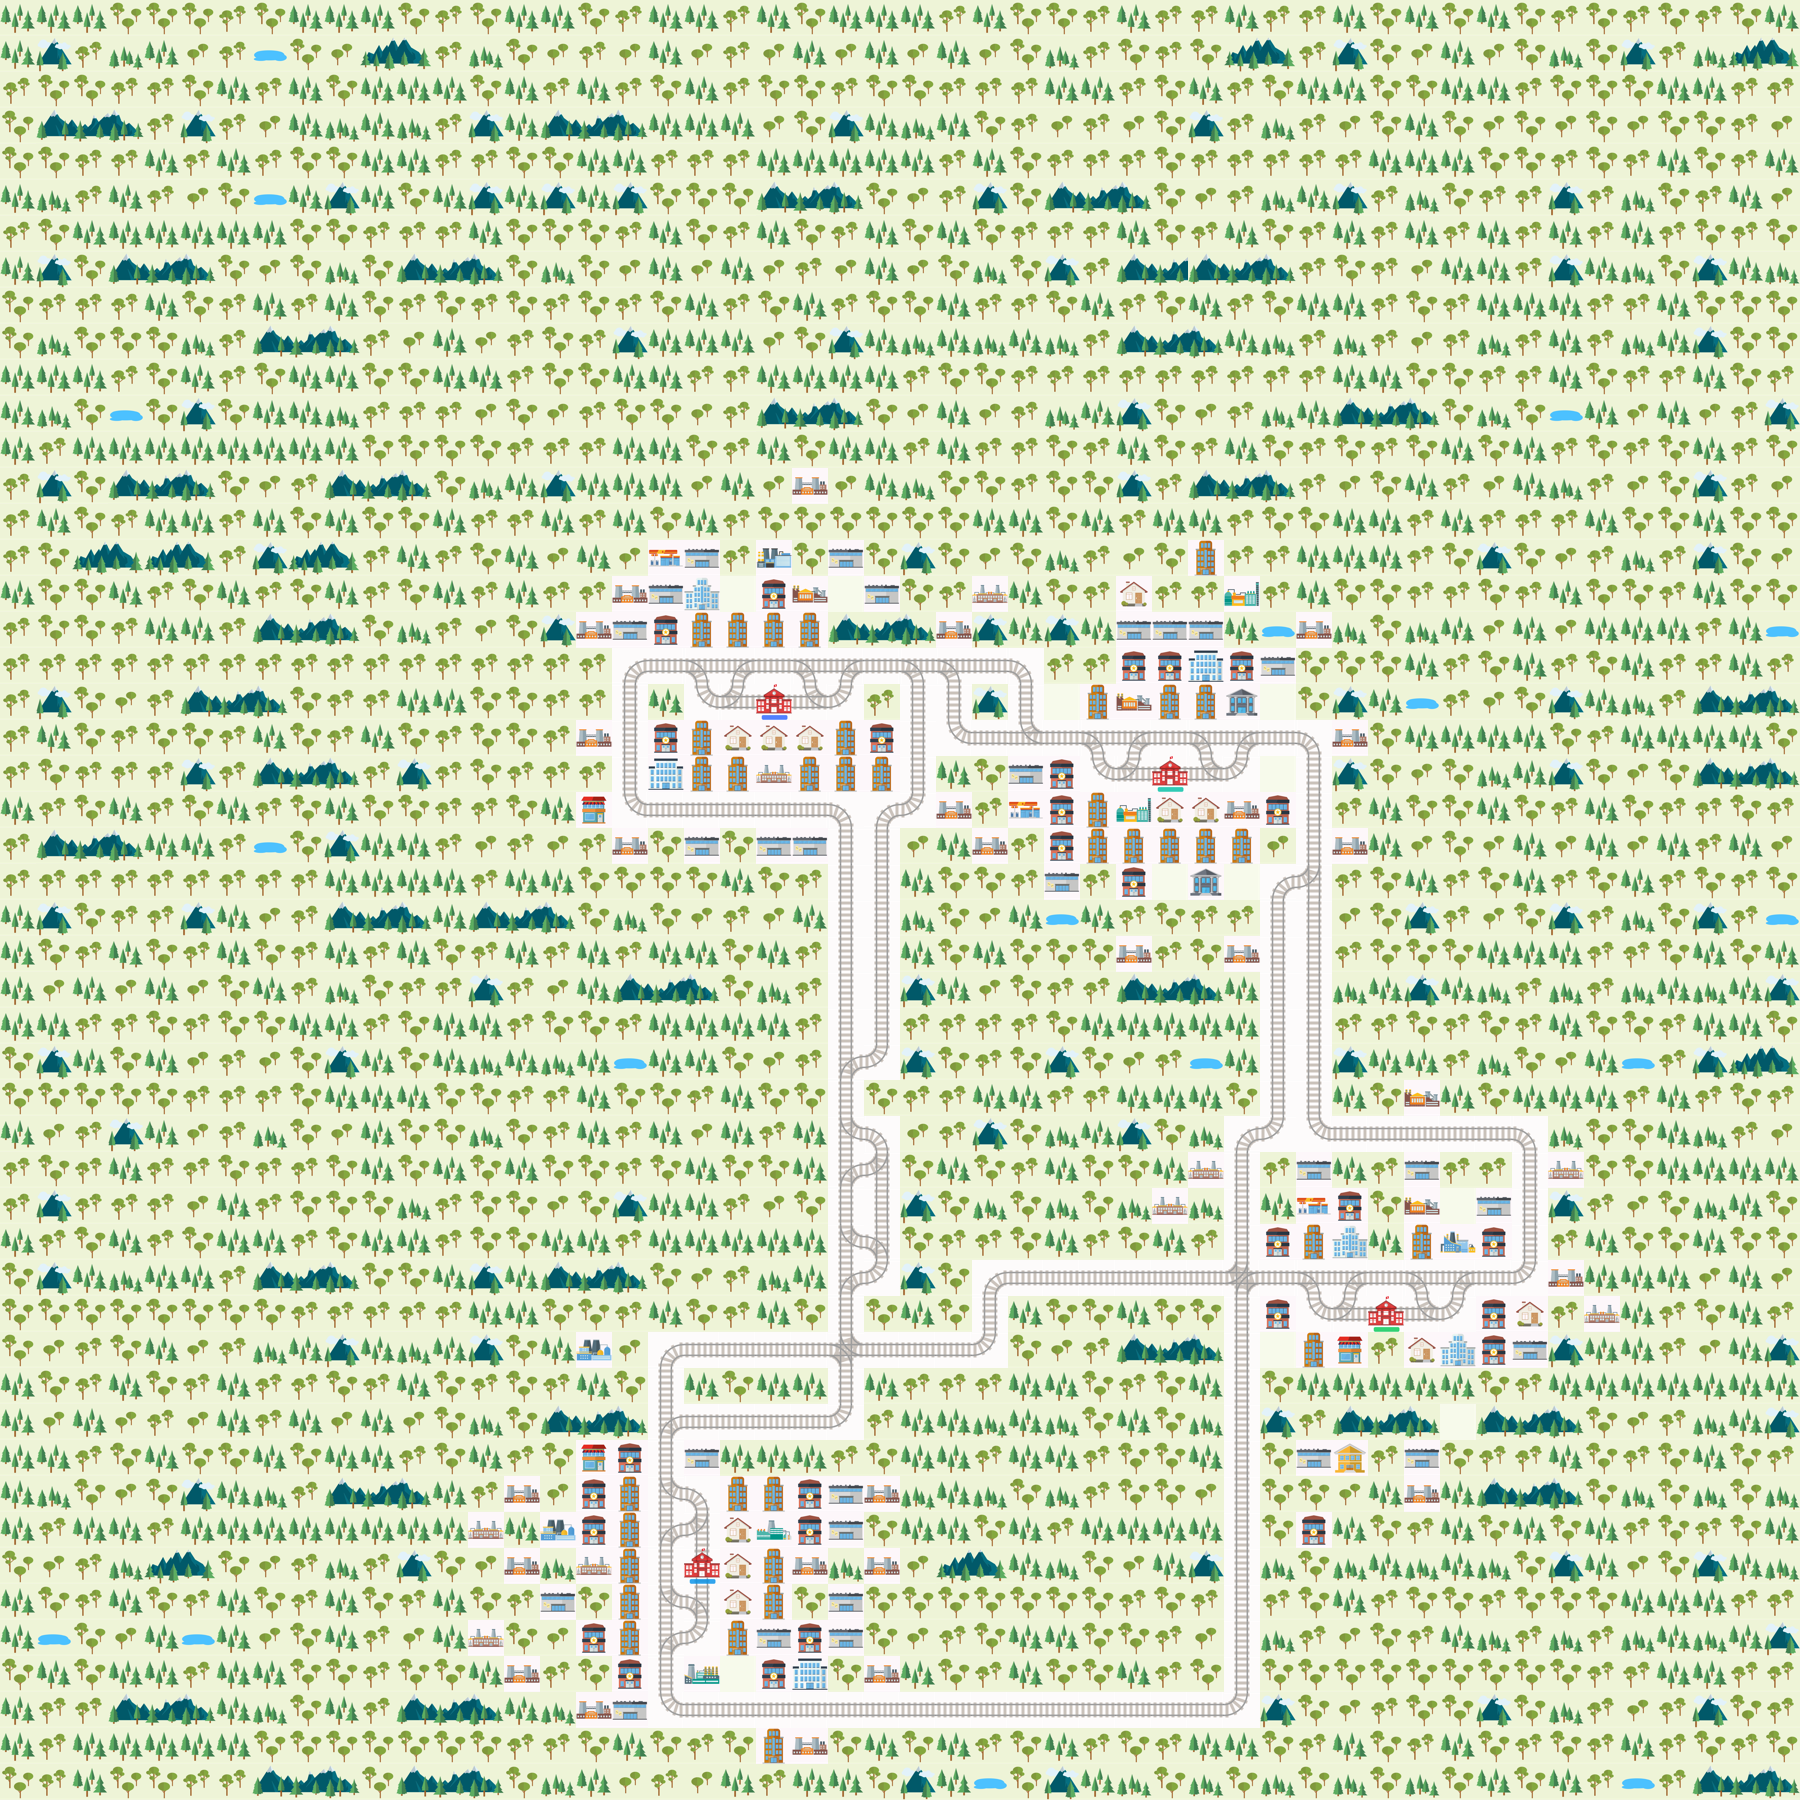
\includegraphics[width=0.9\textwidth]{medium/medium_0_1}
	\caption{Medium instance, using a 50x50 grid, where 10 trains must travel across 5 cities.}
	\label{medium_0_1_fullpage}
\end{figure}


\begin{figure}[h]
	
	\centering
	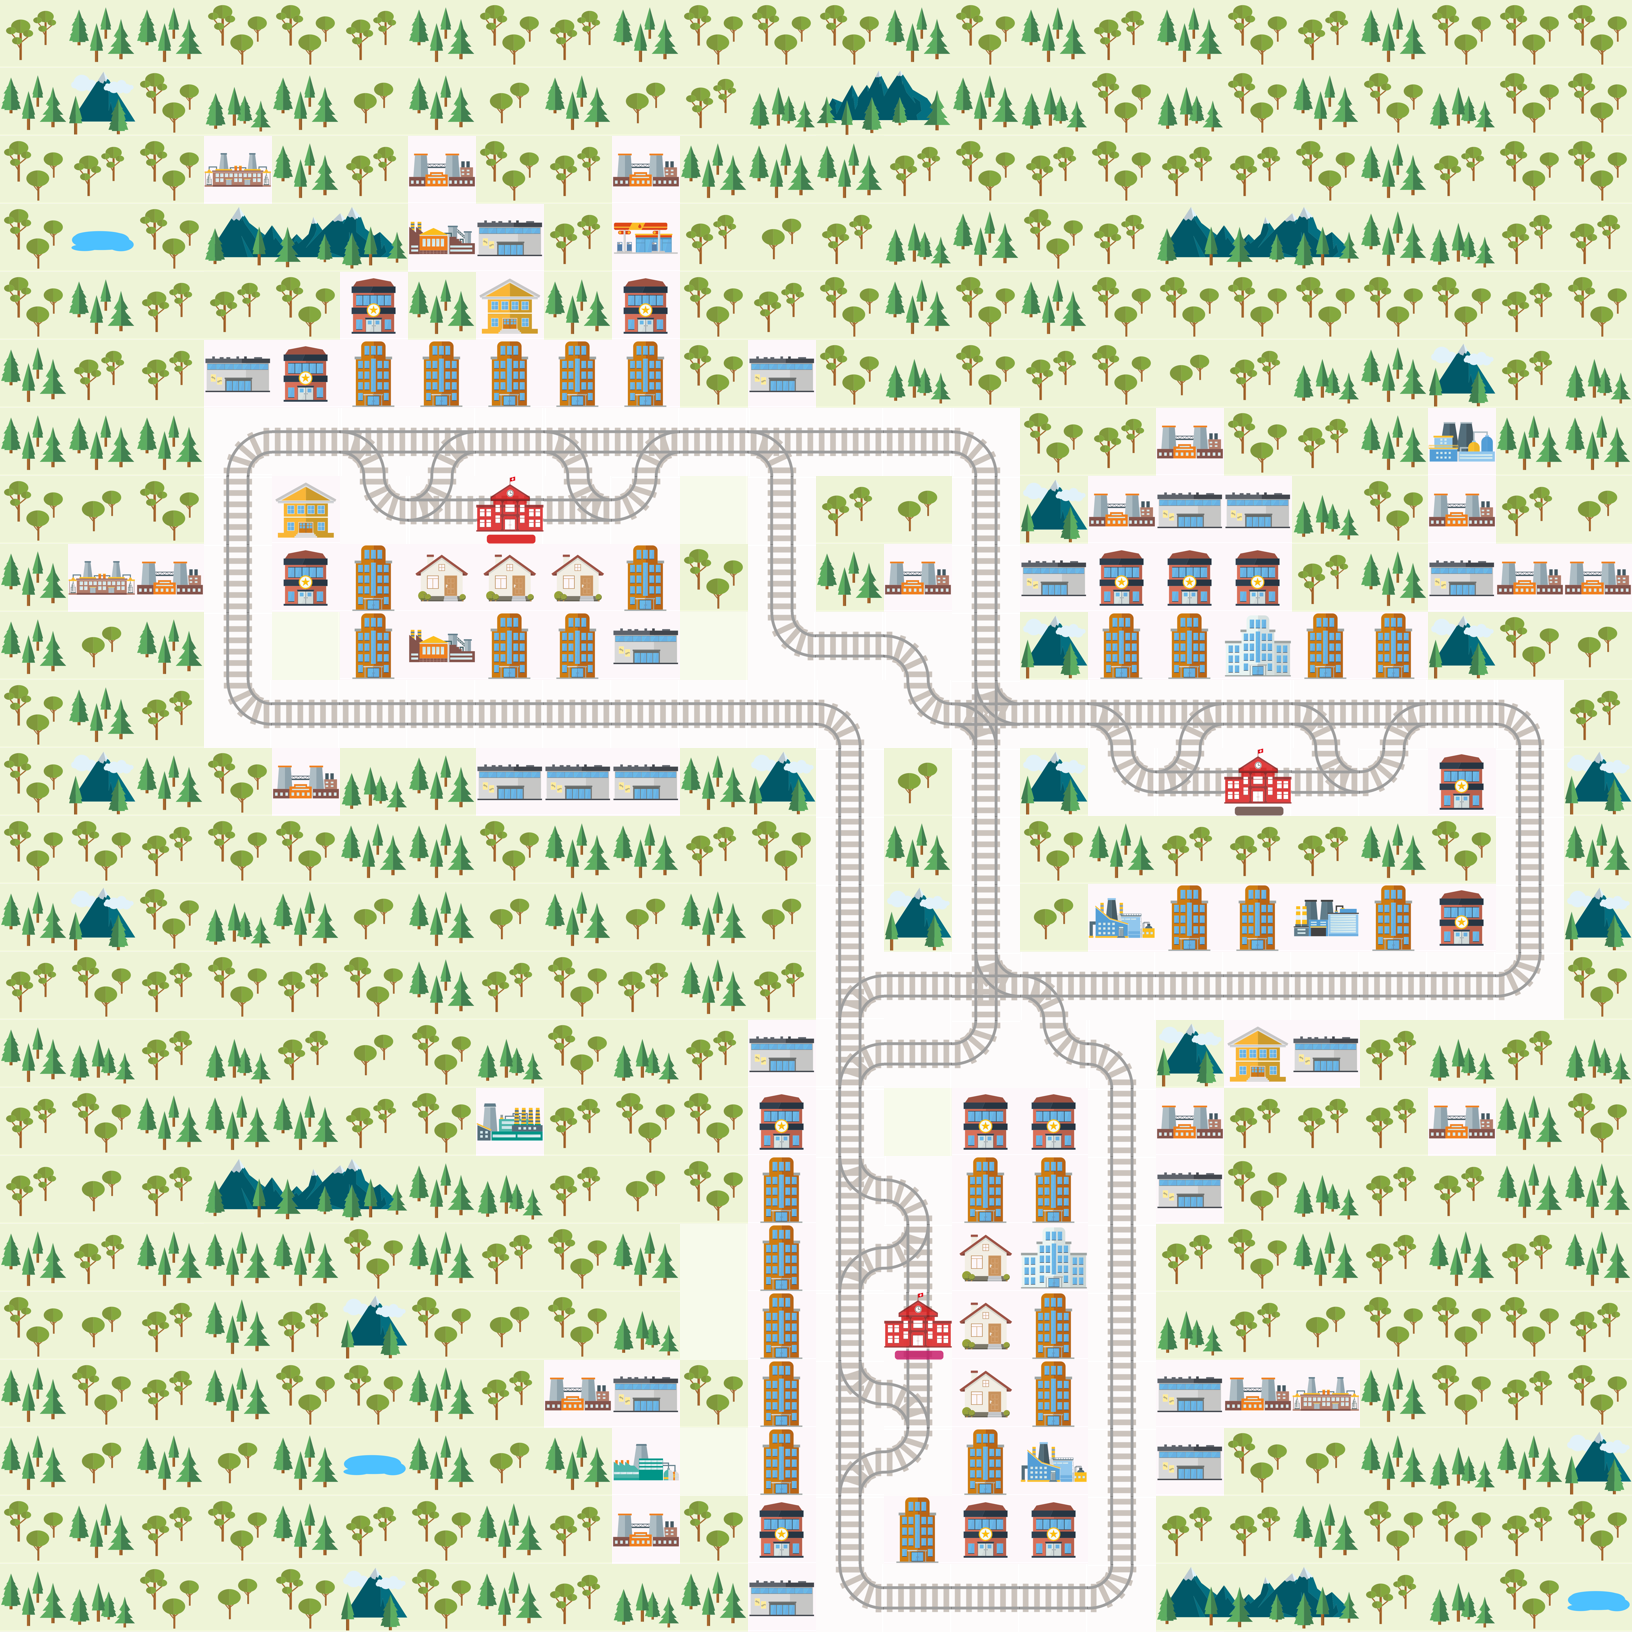
\includegraphics[width=0.9\textwidth]{dense/dense_0_1}
	\caption{Dense instance, using a 24x24 grid, where 20 trains must travel across 3 cities.}
	\label{dense_0_1_fullpage}
\end{figure}



\end{document}
